\documentclass[paper=a4, fontsize=13pt]{article} 
\usepackage[top=1in, bottom=1in, left=1in, right=1in]{geometry}
\usepackage{amstext}
\usepackage{subfigure}
\RequirePackage{graphicx}
\RequirePackage{longtable,multirow,hhline,tabularx,array}
\usepackage[english]{babel} 
\RequirePackage{colortbl,booktabs}
\linespread{1.5}

\title{
\normalfont \normalsize
\huge Battle of Online and Offline Consumption: \\
Comparative Analysis of Amazon and Walmart Stocks
}
\author{Cai Yuzhu, Li Hongchi, Ning Xu, Xue Zheng}
\date{\normalsize\today}

\begin{document}
\maketitle
\section{Introduction}

\section{Data Processing}
In our research report, we use Walmart as the representative of offline seller and Amazon as that of online seller. We focus on the daily log return of the Walmart stock and Amazon stock from January 3th, 2010 to December 30th, 2016, with 1761 observations. All the data are pulled from Wind Financial Terminal.

Let $r_t$ be the log return of an asset at time $t$, and the formula we use to calculate the log return is
\[ r_t = ln(\frac{p_t}{p_{t-1}}) \times 100\% \]
where $p_t$ is the close price in day $t$ and $p_{t-1}$ is the close price in day {t-1}.

The descriptive statistics and time plot are shown in Table \ref{ds} and Firgure \ref{tp}.

\begin{table}[!htbp]
\caption{Descriptive Statistics}  
\centering  
\subtable[Amazon Stock]
{  
\begin{tabular}{ccccc}
  \toprule
  \rowcolor[gray]{.8}
Year & Sample & Mean(\%) & Sd(\%) \\ 
  \midrule
2010 & 251 & 0.1179 & 2.0591 \\ 
2011 & 252 & -0.0155 & 2.4337 \\ 
2012 & 250 & 0.1484 & 1.9656 \\ 
2013 & 252 & 0.1839 & 1.6947 \\ 
2014 & 252 & -0.0995 & 2.0677 \\ 
2015 & 252 & 0.3089 & 2.0582 \\ 
2016 & 252 & 0.0412 & 1.8682 \\ 
2010-2016 & 1761 & 0.0978 & 2.0323 \\ 
   \bottomrule
\end{tabular}
}  
\qquad  
\subtable[Walmart Stock]
{          
\begin{tabular}{ccccc}
  \toprule
  \rowcolor[gray]{.8}
Year & Sample & Mean(\%) & Sd(\%) \\ 
  \midrule
2010 & 251 & 0.0068 & 0.8782 \\ 
2011 & 252 & 0.0515 & 1.0469 \\ 
2012 & 250 & 0.0627 & 1.0309 \\ 
2013 & 252 & 0.0662 & 0.7749 \\ 
2014 & 252 & 0.0445 & 0.8367 \\ 
2015 & 252 & -0.1229 & 1.3191 \\ 
2016 & 252 & 0.0590 & 1.2030 \\ 
2010-2016 & 1761 & 0.0239 & 1.0297 \\ 
   \bottomrule
\end{tabular}
}
\label{ds} 
\end{table}  

\begin{figure}[!htbp]
\begin{minipage}[!htbp]{0.5\linewidth}
\centering
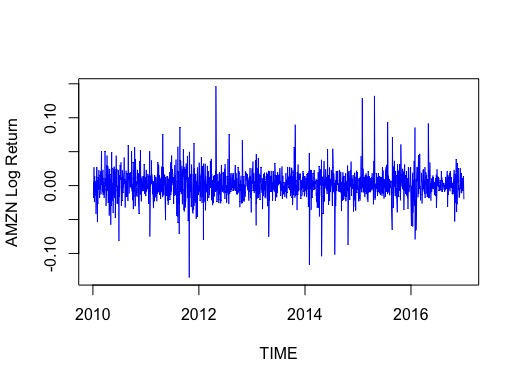
\includegraphics[scale = 0.45]{img/timeplot_AMZN}
\end{minipage}
\begin{minipage}[!htbp]{0.5\linewidth}
\centering
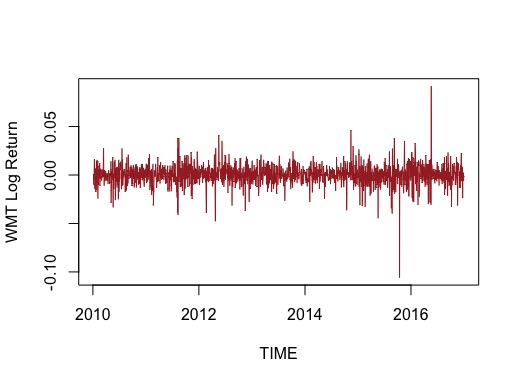
\includegraphics[scale = 0.45]{img/timeplot_WMT}
\end{minipage}
\caption{Timeplots of Amazon (Blue) and Walmart (Red) Stocks}
\label{tp}
\end{figure}

From Table 1, we provide the mean log return and its standard deviation for each stock, and Figure 1 shows the time plots of the log returns for Amazon and Walmart. From the plots, the return series for both stocks appear to be stationary and random.

\section{Model Establishment}
\subsection{Model Specification}
Figure \ref{cf_AMZN}.(a) shows the sample ACF of the log returns for Amazon stock, which suggests no significant serial correlations. Figure \ref{cf_AMZN}.(b), showing the sample PACF of the log returns, also confirms our conclusion of no serial correlation. Then, we plot the sample ACF of the squared log returns for Amazon stock in Figure \ref{cf_AMZN}.(c). Combing the three plots, it seems that the log returns are neither serially correlated nor dependent. Similar results can also be found for Walmart stock in Figure \ref{cf_WMT} that the log returns for Walmart stock are serially uncorrelated and independent.

\begin{figure}[!htbp]
\centering
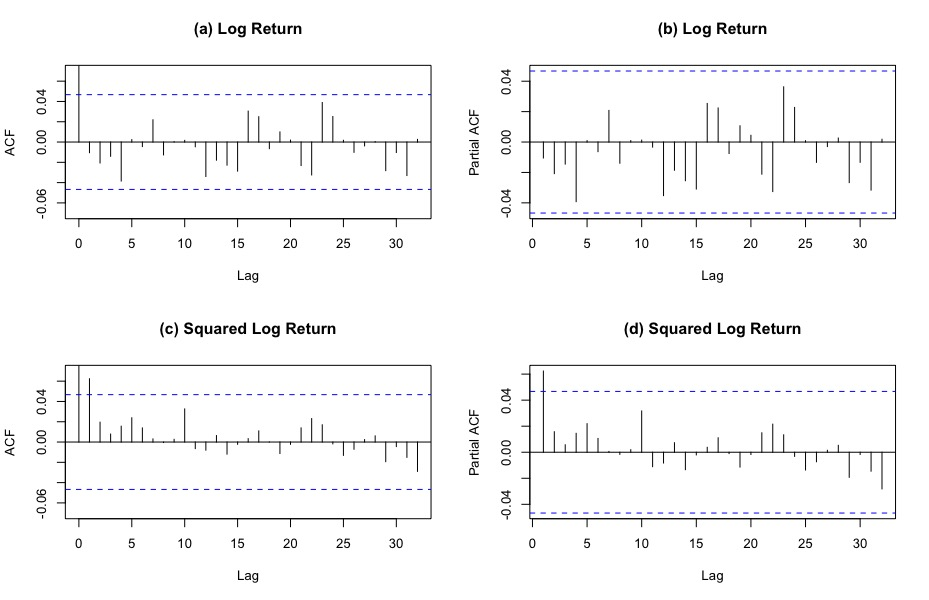
\includegraphics[scale = 0.7]{img/cf_AMZN}
\caption{ACF and PACF of Amazon Stock}
\label{cf_AMZN}
\end{figure}

\begin{figure}[!htbp]
\centering
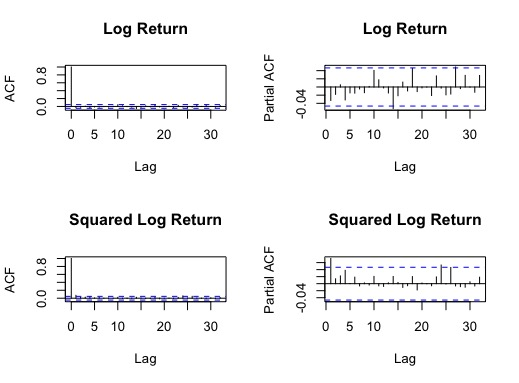
\includegraphics[scale = 0.7]{img/cf_WMT}
\caption{ACF and PACF of Walmart Stock}
\label{cf_WMT}
\end{figure}

\subsection{Mean Equation}
The observations above suggest that the daily log returns of Amazon stock follow an ARMA(0,0) model, in other words, a white noise series. This is in agreement with the result suggested by the sample ACF in Figure 2(c) that all sample ACFs are close to zero. Therefore, we propose a mean equation that is simply a constant plus innovations, $r_t = \mu + a_t$, where $r_t$  is the log return of an asset at time $t$, $\mu$ is the estimate we get using a volatility model. The squared series $a_t^2$ is then used to check for conditional heteroscedasticity (ARCH effects). We perform the usual Ljung–Box statistics Q(m) to the $\{a_t^2\}$ series. The null hypothesis is that the first m lags of ACF of the $a_t^2$ series are zero.

The Ljung–Box statistics of the $a_t^2$ series shows ARCH effects with Q(5) = 9.6519, the p value of which is close to zero.

\subsection{Volatility Equation}
Here we entertain an ARCH(1) model and a GARCH(1,1) model for the volatility and we specify the model as the following:
\[ r_t = \mu+a_t, a_t = \sigma_t \epsilon_t \]
\[ \text{ARCH(1): } \sigma_t^2 = \alpha_0+\alpha_1 a_{t-1}^2 \]
\[ \text{GARCH(1,1): } \sigma_t^2= \alpha_0+\alpha_1 a_{t-1}^2+\beta_1 \sigma_{t-1}^2 \]
in which $\epsilon_t$, here in our model, we assume as a Gaussian innovation that is independent and identically distributed as a Normal distribution with mean 0 and variance 1.

\section{Estimation}

\begin{table}[!htbp] \centering 
  \caption{Ljung-Box tests for ARCH(1) and GARCH(1,1) models for AMZN Stock} 
  \label{} 
\begin{tabular}{cc|cccccc} 
\\[-1.8ex]\hline 
\hline
& & \multicolumn{3}{c}{Standardized residuals} & \multicolumn{3}{c}{Squared standardized residuals} \\
& & Q(10) & Q(15) & Q(20) & Q(10) & Q(15) & Q(20) \\
\hline 
\multirow{2}{*}{ARCH(1)} & statistic & 4.7873 & 10.2395 & 12.8693 & 3.9721 & 4.7376 & 5.1054 \\
& p-value & 0.9049 & 0.8044 & 0.8829 & 0.9486 & 0.9941 & 0.9997 \\
\multirow{2}{*}{GARCH(1,1)} & statistic & 4.1734 & 10.2365 & 12.8473 & 3.0443 & 4.2163 & 4.7107 \\
& p.value & 0.9392 & 0.8046 & 0.8838 & 0.9804 & 0.9969 & 0.9999 \\
\hline
\hline 
\end{tabular} 
\end{table} 

\begin{table}[!htbp] \centering 
  \caption{Results of Estimation of Two Volatility Models for AMZN Stock} 
  \label{} 
\begin{tabular}{@{\extracolsep{5pt}}lcc} 
\\[-1.8ex]\hline 
\hline
 & ARCH(1) & GARCH(1,1) \\ 
\hline \\[-1.8ex] 
 mu & 0.115$^{**}$ & 0.137$^{***}$ \\ 
  & (0.046) & (0.046) \\ 
  & & \\ 
 omega & 3.515$^{***}$ & 1.020$^{***}$ \\ 
  & (0.149) & (0.344) \\ 
  & & \\ 
 alpha1 & 0.168$^{***}$ & 0.129$^{***}$ \\ 
  & (0.036) & (0.032) \\ 
  & & \\ 
 beta1 &  & 0.637$^{***}$ \\ 
  &  & (0.098) \\ 
  & & \\ 
\hline \\[-1.8ex] 
Observations & 1761 & 1761 \\ 
Log Likelihood & 3724.855 & 3720.010 \\ 
Akaike Inf. Crit. & 4.234 & 4.229 \\ 
Bayesian Inf. Crit. & 4.243 & 4.242 \\ 
\hline 
\hline \\[-1.8ex] 
\textit{Note:}  & \multicolumn{2}{r}{$^{*}$p$<$0.1; $^{**}$p$<$0.05; $^{***}$p$<$0.01} \\ 
\end{tabular} 
\end{table} 

Based on the results of log likelihood, AIC, and BIC for ARCH(1) model and GARCH(1,1) model, GARCH(1,1) is slightly more appropriate.

Consequently, we obtain a GARCH(1,1) to model the volatility:
\[ \sigma_t^2 = 1.0199+0.1286 a_{t-1}^2+0.6373\sigma_{t-1}^2 \]

where the standard errors of the parameters are 0.3435, 0.0315, 0.0984, respectively.

In conclusion, we propose the following mean equation and conditional heteroskedasticity model for AMZN stock
\[ r_t = 0.1367+a_t, \sigma_t^2 = 1.0199+0.1286a_{t-1}^2+0.6373\sigma_{t-1}^2. \]

\begin{table}[!htbp] \centering 
  \caption{Ljung-Box tests for ARCH(1) and GARCH(1,1) models for WMT Stock} 
  \label{} 
\begin{tabular}{cc|cccccc} 
\\[-1.8ex]\hline 
\hline
& & \multicolumn{3}{c}{Standardized residuals} & \multicolumn{3}{c}{Squared standardized residuals} \\
& & Q(10) & Q(15) & Q(20) & Q(10) & Q(15) & Q(20) \\
\hline 
\multirow{2}{*}{ARCH(1)} & statistic & 9,0085 & 15.1256 & 20.0360 & 2.1312 & 2.4483 & 4.4991 \\
& p-value & 0.5313 & 0.4424 & 0.4557 & 0.9952 & 0.9999 & 0.9999 \\
\multirow{2}{*}{GARCH(1,1)} & statistic & 8.8064 & 14.4575 & 18.5378 & 1.6428 & 1.9398 & 4.0184 \\
& p.value & 0.5506 & 0.4912 & 0.5520 & 0.9984 & 0.9999 & 0.9999 \\
\hline
\hline 
\end{tabular} 
\end{table} 

\begin{table}[!htbp] \centering 
  \caption{Results of Estimation of Two Volatility Models for WMT Stock} 
  \label{} 
\begin{tabular}{@{\extracolsep{5pt}}lcc} 
\\[-1.8ex]\hline 
\hline
 & ARCH(1) & GARCH(1,1) \\ 
 mu & 0.037 & 0.033 \\ 
  & (0.023) & (0.024) \\ 
  & & \\ 
 omega & 0.863$^{***}$ & 0.442$^{**}$ \\ 
  & (0.036) & (0.187) \\ 
  & & \\ 
 alpha1 & 0.192$^{***}$ & 0.140$^{***}$ \\ 
  & (0.034) & (0.040) \\ 
  & & \\ 
 beta1 &  & 0.445$^{**}$ \\ 
  &  & (0.207) \\ 
  & & \\ 
\hline \\[-1.8ex] 
Observations & 1761 & 1761 \\ 
Log Likelihood & 2506.755 & 2506.020 \\ 
Akaike Inf. Crit. & 2.850 & 2.851 \\ 
Bayesian Inf. Crit. & 2.860 & 2.863 \\ 
\hline 
\hline \\[-1.8ex] 
\textit{Note:}  & \multicolumn{2}{r}{$^{*}$p$<$0.1; $^{**}$p$<$0.05; $^{***}$p$<$0.01} \\ 
\end{tabular} 
\end{table} 

Following the same logic as in the previous section, we select ARCH(1) model for WMT Stock. Since there’s little difference between these two models based on their log likelihood, AIC, and BIC, our selection is rather subjective.

Consequently, we obtain a ARCH(1) to model the volatility:
\[ \sigma_t^2 = 0.1286+0.1920 a_{t-1}^2 \]

where the standard errors of the parameters are 0.0358, and 0.03389, respectively.

In conclusion, we propose the following mean equation and conditional heteroskedasticity model for AMZN stock
\[ r_t = 0.0372+a_t, \sigma_t^2 = 0.1286+0.1920a_{t-1}^2. \]

\section{Model Checking}

\section{Prediction}

\section{Conclusion}

\section{Appendix}

\begin{thebibliography}{99}
\bibitem{1} hahahahahahahaha
\end{thebibliography}


\end{document}
